\chapter{Descripción implementación}

\section{Limitaciones técnicas}
\label{sec:limitaciones-tec}
Antes de iniciar con la implementación del esquema de anotación propuesto, tanto
para las clases de la API \ref{subsec:api}, como para los aplicativos a analizar
\ref{subsec:apps}, se identifican una serie de limitaciones del lenguaje
Jif para anotar código de la API de Android. 
Tales limitaciones son adicionales a las características del lenguaje Java no
soportadas por Jif, a continuación se describen tanto las encontradas, como las
especificadas en el manual de referencia de Jif.

\subsection{Características del lenguaje Java no soportadas por jif}
% -\textit{Características del lenguaje Java no soportadas por jif}\newline
Si bien, el sistema de anotaciones de Jif hace extensiones al lenguaje java,
permitiendo la evaluación de políticas de confidencialidad e integridad para
aplicativos implementados en dicho lenguaje, el manual de referencia de Jif
precisa las características del lenguaje Java no soportadas\cite{jifRef}. Estas
son:
\begin{itemize}
  \item nested classes: clases que son definidas dentro de otras clases.
  \item initializer blocks: bloques de código declarados dentro de la clase pero
  sin pertenecer a ningún método, dependiendo de si se trata de static
  initialization blocks, su código es el primero en ejecutarse, una vez se
  carga la clase; o si se trata de instance initialization blocks, su código se
  ejecutan cada vez que se crea una instancia de la clase.
\item threads.
\end{itemize} 
Partiendo de estas precisiones, aplicaciones Android que presenten tales
características son excluidas del grupo de aplicaciones a analizar(conjunto de
aplicaciones evaluables) mediante la herramienta propuesta.

% Adicional a las limitaciones de jif frente a características propias del
% lenguaje Java, tras experimentar la anotación manual de una serie de
% aplicaciones Android, se identifican varias limitaciones técnicas para la
% anotación de de las mismas. Entre las limitaciones identificadas están:\newline 
\subsection{Soporte para la clase java.lang.Override}
\label{sub:override}
% - \textit{Soporte para sobreescritura de métodos}\newline 
En la construcción de aplicaciones Android, según el componente que se esté
implementando(activities, content providers, receivers, services), se requiere
sobreescribir métodos de la clase que extienda el componente. Así, cuando se
define un componente tipo Activity, que debe extender de la clase Activiy.java, 
se sobreescriben métodos como Oncreate. Cada que se sobreescribe
un método se utiliza el statement @Override, con el cual se informa al
compilador de Java que el método es sobreescrito. No obstante, al implementar la
versión Jif de aplicaciones Android con dicho statement, el compilador de Jif
no lo reconoce. La dificultad que se presenta está en el reconocimiento del
statement(carácter @ y clase Override), y no en la sobreescritura de métodos,
puesto que Jif soporta tal característica.\newline 
El soporte para la sobreescritura de
métodos es confirmado con una sencilla prueba, anotando la clase Activity.java
del framework Android (con un único método, el método Ocreate), e implementando
la versión Jif de una aplicación Android que extiende de tal clase, en la cual
se define una actividad y sobreescribe el método Oncreate.
Cuando se comenta la sentencia @Override, el compilador de Jif identifica la
sobreescritura del método y reporta comentarios para el flujo de información.

Al investigar el por qué Jif no reconoce tal sentencia, se encuentra que dentro
de las clases Java estándar soportadas por el compilador de Jif, no se incluye
la clase java.lang.Override.\newline 
Las clases Java estándar pertenecientes a los paquetes io, lang, math, net y
sql; soportadas po el compilador Jif, vienen implementadas con anotaciones en el
directorio sig-src, directorio que forma parte de la distribución del compilador
de Jif con que se esté trabajando.

Un mecanismo para permitir el análisis de flujo de información entre métodos
que se sobreescriben, es comentar las líneas del programa que contengan la
sentencia @Override, puesto que, al no ser reconocida por el compilador de Jif,
es la generadora de errores de compilación.

\subsection{Casting entre tipos EditText y View}
\label{sec:casting}
El framework de Android cuenta con diferentes clases para manejar las interfaces
gráficas que presenta al usuario, entre las cuales se encuentran EditText y
View.\newline
View es la clase principal para la creación de widgets, necesarios para la
implementación de componentes interactivos en las interfaces de
usuario(UI).\newline 
EditText permite adicionar campos de texto editables en UI.\newline
El casting entre los tipos de datos que representan ambas clases, se hace cuando la aplicación debe
procesar datos provenientes de campos en las interfaces del usuario, por ejemplo
como se observa a continuación:
\begin{lstlisting}
EditText editPassword = (EditText)findViewById(R.id.password);
String password = editPassword.getText().toString();
\end{lstlisting}
la interfaz de usuario(que es de tipo View) contiene un campo R.id.password, y
para manipular la información que almacena, debe ser de tipo EditText, siendo
necesario un casting de tipo View a tipo EditText. La dificultad que se presenta
con este tipo de casting es que para el sistema de anotaciones de jif no es
válido. Luego de probar con la anotación manual de ambas clases, tratando de
dar soporte a este tipo de casting, sin obtener resultados satisfactorios, se
opta por ``simular'' estos casos, es decir, si el tipo de dato de una variable
es de tipo EditText, se crea una variable tipo String con un valor determinado,
así se omite el casting y se puede analizar el flujo de información.

\subsection{Clase nested R}
\label{sec:nested}
El framework de Android utiliza identificadores para hacer referencia a recursos
utilizados por la aplicación, recursos como strings, estilos, widgets, layouts, e
interfaces xml, tales identificadores son autogenerados en la clase R.java, allí
cada recurso es descrito como una clase individual. Al tratarse de una clase
nested, la clase R no puede ser anotada con jif. Esto puede solucionarse
implementando una versión Jif generalizada de la clase R, que contenga los
recursos utilizados en una aplicación, definidos como variables y no como clases.

% - \textit{Sources y Sinks}\newline
% En los preliminares para el diseño de la solución se propone utilizar SuSi
% para clasificar los sources y sinks en las aplicaciones a analizar, sin embargo, partir del
% extenso conjunto de sources y sinks, clasificados por SuSi para la API de
% Android, implica una mayor complejidad en el análisis, puesto que, en un
% aplicativo todo el código que le conforma puede hacer parte de sources o de
% sinks. Adicional a lo complejo que se puede tornar el análisis, los sources y
% sinks a considerar deben depender de la política de seguridad a evaluar. En ese
% orden de ideas, resulta más viable tomar un subconjunto del listado proveído por
% SuSi, partiendo de los sources y sinks que evalué la política de seguridad que
% se defina.

\subsection{Enhanced for loop}
\label{seubsec:enh}
Además de soportar la estructura de control for, el lenguaje Java permite el uso
de enhanced for, que es utilizado para simplificar la iteración en arrays y
colecciones, por ejemplo:
% \begin{lstlisting}
% char c[] = imei.toCharArray();
% for (int i = 0; i < c.length; i++) {
% 	obfuscated += c[i] + "_";
% }          
% \end{lstlisting}  
\begin{lstlisting}
for(char c : imei.toCharArray())
obfuscated += c + "_";
\end{lstlisting}
A diferencia de Java, Jif no soporta el enhanced for.\newline
Debido a que ambas sentencias de control son equivalentes, la solución que se
propone para poder analizar flujo de información en los aplicativos Android que
contengan dicha estructura de control, es generar el equivalente del programa
haciendo uso del for, de este modo se cambia la sintaxis sin afectar la lógica
del aplicativo a analizar.

\subsection{Otras limitaciones}
Adicional a las limitaciones descritas anteriormente, para las cuales se propone
una solución, se identifica que Jif no soporta la sintaxis utilizada para
definir estructuras de datos HashMaps, LinkedList y Sets, que en Java se definen
de la siguiente manera:
\begin{lstlisting}
Map<String,String> hashMap = new HashMap<String, String>();
List<String> listData;
Set<String> phoneNumbers = new HashSet<String>();
\end{lstlisting}
Jif tampoco permite la definición de interfaces como argumentos de un método. El
siguiente fragmento de código  en una aplicación Android, muestra la definición
de una interfaz pasada como parámetro al método setOnClickListener.
\begin{lstlisting}
   Button button1= (Button) findViewById(R.id.button1);
   button1.setOnClickListener(new View.OnClickListener() {
   ...
   .....}  });
\end{lstlisting}
En estos casos, la dificultad está en encontrar una sintaxis que permita obtener
la versión equivalente del programa que las contenga. A lo que se suma, la falta
de documentación disponible para solventar los mismos. En consecuencia, se omite
del conjunto de aplicaciones evaluables, aplicaciones Android que requieran en
su implementación las estructuras de datos descritas.\newline

%- \textit{Paso de statements dentro de los argumentos de un método
%(\{\}):}\newline
\section{Detalles de implementación}
Como se describió anteriormente, la implementación del diseño requiere
anotaciones a la API de Android y anotaciones en los aplicativos a
analizar.\newline 
En el caso de las anotaciones requeridas para la API \ref{subsec:api},
su anotación se hace manualmente.\newline 
En el caso de las anotaciones en el
aplicativo a analizar \ref{subsec:apps}, para las que se propuso un esquema de anotación automatizable, se implementa un
prototipo de anotación en lenguaje Java. En la sección \ref{sec:diagramaClass}
de los anexos, se incluye su respectivo diagrama de clases.\newline 
El anotador está implementado en lenguaje Java y consta de cinco clases:
\emph{Main}, \emph{Source}, \emph{XmlExtract}, \emph{Annotation} y
\emph{BufferWriter}.\newline 
Todos los pasos de anotación descritos en
\ref{subsec:pasosSol}, son coordinados desde la clase \emph{Main}.\newline
La clase \emph{Source} identifica qué variables source contiene la aplicación que se
está analizando, esta clase se apoya en la clase \emph{XmlExtract} para identificar
sources definidos en interfaces UI. En este caso particular, para la
verificación de la política establecida, la clase \emph{XmlExtract} permite identificar
el source EditText, cuando se trata de un campo UI que almacena
contraseñas.\newline 
Como las interfaces UI se describen mediante XML, es
necesario extraer los elementos de la interfaz utilizando las librerías javax.xml.parsers y
org.w3c.dom. Con javax.xml.parsers se obtiene el respectivo DOM del XML a
analizar. Con org.w3c.dom se recorren los elementos del DOM, elementos como los
campos EditText.\newline 
Con la clase \emph{Annotation}  se identifican y anotan los diferentes tipos de
métodos(métodos source, no source y métodos a sobreescribir).\\
En la clase \emph{BufferWriter} se anotan las variables sources, y finalmente
se retorna la versión .jif del aplicativo que se está analizando.\newline 
Para la anotación del código se utiliza la librería Java Parser 1.8  que permite
generar y visitar el árbol de sintaxis para la estructura del código de cada
programa, haciendo posible la adición de los labels de seguridad respectivos.\\
% \textcolor{blue}{(Incluir Figura)}\newline 
\label{subsec:anotador}
\begin{figure}[t!]
	\begin{center}
	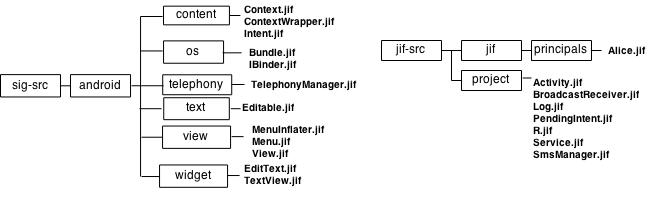
\includegraphics[width=12cm]{JifFilesystem.jpg}
	\end{center}
	\caption{Estructura de directorios en Jif.
	El código con anotaciones que se requiere para la evaluación de flujo de
	información en Jif, es alojado en los directorios sig-src y jif-src.}
	\label{fig:jifFilesystem} 
\end{figure}

\section{Ambiente y herramientas}
\textit{Versión de la API de Android}\newline
Las anotaciones a las clases de la API Android y las aplicaciones a anotar
mediante el prototipo, corresponden a la versión Android 4.2.2(API Level 17).

\textit{Versión del compilador de Jif}\newline
El componente que verifica el cumplimiento de las políticas de seguridad,
corresponde a la versión 3.4.2 del compilador de Jif.

\textit{Estructura de trabajo en JIF}\newline
El compilador de Jif maneja una estructura de directorios en la que se incluye
el código fuente .jif de las aplicaciones a analizar. Como ilustra la figura
\ref{fig:jifFilesystem} se tienen los directorios principales sig-src y jif-src.
El directorio sig-src está destinado para incluir librerías adicionales.\newline 
El directorio jif-src contiene todo el código jif correspondiente al programa
como tal que se va evaluar mediante Jif. Para los propósitos del presente
trabajo, se tienen los subdirectorios principals y project. En el subdirectorio
principals se incluyen las autoridades requeridas, y en el subdirectorio
project se incluyen, tanto las clases específicas de los aplicativos Android a
analizar, como las clases de que estos heredan como: Activity.jif, Service.jif,
etc.

\section{Compilación, integración y finalmente ejecución }
Las instrucciones para ejecutar la herramienta de análisis que se propone son
descritas en la sección \ref{sec:ejecutarPrototipo} de los anexos, allí se
ilustra paso a paso cómo ejecutar el anotador, y cómo compilar los aplicativos
a analizar mediante Jif.
